\author{Martin Hausleitner}
\section{Technologieevaluierung}

Ein zentraler Aspekt jedes Projektbeginns ist die Evaluierung der Technologie. Wir haben uns bewusst viel Zeit genommen, um eine schnelle und unkomplizierte Entwicklung zu ermöglichen und später mögliche Bedauern zu vermeiden. Die Anforderungen für das Projekt umfassen die Erstellung von iOS- und Android-Apps sowie möglicherweise einer Web-App in Zukunft. Hinsichtlich des Backends ist für uns insbesondere die Unterstützung von Geopoints und Geo-Queries in der Datenbank von Bedeutung. Idealerweise sollte das System zudem eine integrierte Authentifizierungsfunktion aufweisen.


\subsection{Frontend}

Im Bereich der Frontend-App-Entwicklung stehen verschiedene Möglichkeiten zur Verfügung, um eine App zu programmieren. Eine Option besteht darin, eine nativ programmierte iOS- oder Android-App zu erstellen. Allerdings haben wir uns als Team schnell gegen diese Option entschieden, da keiner von uns mit einer der Plattformen vertraut ist und dies zu einem erheblichen Mehraufwand führen würde. Dies würde bei einem kleinen Team von nur drei Personen zu viel Zeit in Anspruch nehmen. Ein Vorteil der nativen Programmierung besteht jedoch darin, dass man auf alle nativen APIs zugreifen kann und die Performance besser ist, da die Entwickler der App-Schnittstelle vom Hersteller des Betriebssystems stammen.

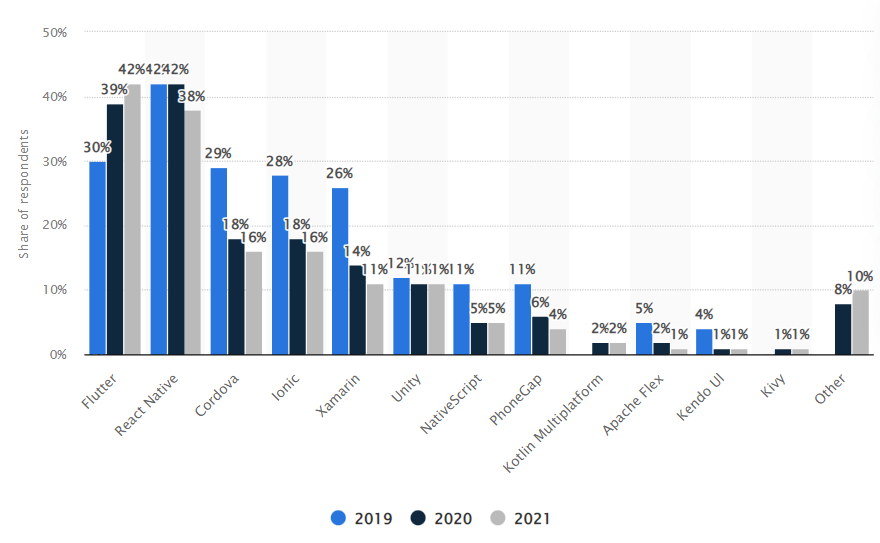
\includegraphics[width=0.75\textwidth]{pics/cross-platform-statisitics.png}
https://www.statista.com/statistics/869224/worldwide-software-developer-working-hours/


\begin{tabular}{|@{Row:}l|c||r|}
    Left Top (no left margin)    & Center Top    & Right Top    \\
    Left Bottom (no left margin) & Center Bottom & Right Bottom
\end{tabular}
\begin{table}[]
    \begin{tabular}{l}
        \textbackslash{}begin\{table\}                                                                                                                                \\
        \textbackslash{}centering                                                                                                                                     \\
        \textbackslash{}begin\{tabular\}\{|l|c|c|\}                                                                                                                   \\
        \textbackslash{}hline                                                                                                                                         \\
        \textbackslash{}textbf\{Kriterium\} \& \textbackslash{}textbf\{Appwrite\}          \& \textbackslash{}textbf\{Firebase\} \textbackslash \textbackslash{}hline \\
        Skalierbarkeit     \& Gut                        \& Sehr gut \textbackslash \textbackslash{}hline                                                             \\
        Echtzeit-Datenbank \& Unterstützt                \& Unterstützt \textbackslash \textbackslash{}hline                                                          \\
        Business-Logik     \& Gut                        \& Sehr gut \textbackslash \textbackslash{}hline                                                             \\
        Authentifizierung  \& Einfach                    \& Einfach \textbackslash \textbackslash{}hline                                                              \\
        Geoqueries         \& Unterstützt                \& Unterstützt \textbackslash \textbackslash{}hline                                                          \\
        Storage            \& Unterstützt                \& Unterstützt \textbackslash \textbackslash{}hline                                                          \\
        Cloud-Funktionen   \& Ja                         \& Ja \textbackslash \textbackslash{}hline                                                                   \\
        Flutter-SDKs       \& Ja                         \& Ja \textbackslash \textbackslash{}hline                                                                   \\
        Preis              \& Kostenlos bis 1.000 Nutzer \& Kostenlos bis 10.000 Lese- und 20.000 Schreibvorgänge pro Tag \textbackslash \textbackslash{}hline        \\
        \textbackslash{}end\{tabular\}                                                                                                                                \\
        \textbackslash{}caption\{Vor- und Nachteile von Appwrite und Firebase\}                                                                                       \\
        \textbackslash{}label\{tab:eval:tech\}                                                                                                                        \\
        \textbackslash{}end\{table\}
    \end{tabular}
\end{table}

Nach ausführlicher Recherche wurden die folgenden plattformübergreifenden Frameworks in Betracht gezogen\cite{cross_platform_framework_comparison}: Flutter, React Native, Ionic und Xamarin. Jede Plattform hat ihre Vor- und Nachteile.

Nach langer Recherche und Evaluierung aller Faktoren wurde Flutter als Plattform für das Frontend ausgewählt. Insbesondere das schnelle entwicklung und das einfache Debugging sowie die Integration in VS Code waren entscheidende Faktoren. Jeder aus unserem Team hat eine eigene Flutter Test App programmiert \cite{flutter_test_apps} um die entscheidung zu festigen.

Insgesamt waren wir mit unserer Entscheidung, Flutter zu verwenden, sehr zufrieden. Während der Entwicklungszeit stellte sich heraus, dass die Klammerverwendung in Flutter am Anfang etwas ungewohnt war, aber dank der hervorragenden Unterstützung durch die Flutter-Community und der umfangreichen Dokumentation auf Stack Overflow konnten wir alle Herausforderungen bewältigen. Außerdem wurde die Entwicklung durch die ständigen Verbesserungen und Updates von Flutter, wie der Einführung der Impeller-Rendering-Engine, beschleunigt. \cite{flutter_impeller}

Insgesamt war die Wahl von Flutter für das Frontend der App eine gute Entscheidung.

\subsection
{Backend}

% Für die Implementierung einer mobilen App in Flutter für die Diplomarbeit von Martin Hausleitner wurden verschiedene Backend-Technologien evaluiert. Dabei wurden folgende Anforderungen an die Technologie gestellt: Skalierbarkeit, Realtime-Datenbank für Chat, Business-Logik für den Beitragsradius, sichere Authentifizierung und Verschlüsselung sowie eine einfache und schnelle Entwicklungsmöglichkeit.

% Die drei Favoriten für die Backend-Technologie waren Supabase \cite{supabase}, Firebase\cite{firebase} und Appwrite\cite{appwrite}. Diese wurden alle zum damaligen Zeitpunkt (Februar 2022) mit einem Flutter-SDK unterstützt.

% Technologieevaluation für eine Diplomarbeit

% Die Wahl der richtigen Technologie für eine Diplomarbeit ist von entscheidender Bedeutung für den Erfolg des Projekts. In diesem Abschnitt werden verschiedene Technologien zur Umsetzung einer Chat-App evaluiert.

% Zu den wichtigsten Anforderungen an die Technologie gehören Skalierbarkeit, Echtzeit-Datenbank für den Chat, eine robuste Business-Logik für den Beitragsradius, sichere Verschlüsselung und eine einfache Entwicklung.

Für unser Projekt kamen drei Technologien in frage: Supabase \cite{supabase}, Firebase\cite{firebase} und Appwrite\cite{appwrite} Sie alle bieten SDKs für Flutter und verfügen über eine benutzerfreundliche Authentifizierungsschicht. Darüber hinaus verfügen sie alle über eine Datenbank, die Geoqueries für das Hauptfeature des Beitragradius unterstützt, sowie einen Speicherplatz für Beitragsfotos.

Allerdings bietet Supabase zum Zeitpunkt der Evaluierung im Februar 2022 noch keine Cloud-Funktionen wie Firebase und Appwrite, was es schwierig macht, eine robuste Business-Logik umzusetzen. Obwohl Supabase am 1. April 2022 experimentell Edge Functions eingeführt hat, ist dies für eine Produktions-App nicht empfehlenswert.

Daher wurden Appwrite und Firebase als die beiden besten Optionen identifiziert. Firebase bietet bessere Flutter-SDKs und verfügt über mehr Features, einschließlich der Unterstützung von Google für Flutter, weshalb wir uns schließlich für Firebase entschieden haben.

In der folgenden Tabelle sind die Vor- und Nachteile von Appwrite und Firebase aufgeführt:










% \begin{table}[h]
%     \centering
%     \begin{tabular}{|p{4cm}|p{6cm}|p{6cm}|}
%         \hline
%                   & \textbf{Firebase}                                                                        & \textbf{Appwrite} \ \hline
%         Vorteile  & \begin{itemize}
%                         \item Gute Dokumentation
%                         \item Einfache Integration mit Flutter-SDKs
%                         \item Umfangreiche Features wie Analytics, Performance Monitoring, Cloud Messaging, etc.
%                         \item Schnelle und einfache Entwicklung
%                     \end{itemize}
%                   &
%         \begin{itemize}
%             \item Open Source
%             \item Einfache Integration mit Flutter-SDKs
%             \item Sichere Authentifizierung und Verschlüsselung
%             \item Einfache Skalierbarkeit
%             \item Bietet auch Serverless-Funktionen
%         \end{itemize} \ \hline
%         Nachteile & \begin{itemize}
%                         \item Kostenpflichtig bei Nutzung größerer Mengen an Ressourcen
%                         \item Abhängigkeit von Google
%                     \end{itemize}
%                   &
%         \begin{itemize}
%             \item Weniger umfangreiche Features als Firebase
%             \item Keine direkte Integration mit anderen Google-Tools
%         \end{itemize} \ \hline
%     \end{tabular}
%     \caption{Vor- und Nachteile von Firebase und Appwrite}
%     \label{tab:impl:backend}
% \end{table}

Insgesamt bietet Firebase aufgrund der umfangreichen Features und der einfacheren Integration mit anderen Google-Tools Vorteile gegenüber Appwrite.


\section{Fazit}

Die Wahl von Flutter als Frontend-Plattform und Firebase als Backend-Plattform erwies sich als gute Entscheidung für die Anforderungen dieser Diplomarbeit. Die Einfachheit der Syntax, das schnelle Debugging und die umfangreiche Dokumentation und Unterstützung durch die Community machten Flutter zu einer einfachen und effizienten Plattform für die Entwicklung der mobilen Apps. Firebase hat eine gute Lösung für die Echtzeit-Datenbank und die Geodatenbank und eine einfache Integration mit Flutter.

Insgesamt haben die gewählten Technologien dazu beigetragen, dass die Entwicklung der Anwendung schnell und effizient verlief und die Anforderungen der Diplomarbeit erfüllt wurden.

